\section{Energetic particles in the heliosphere}
\label{sec:particles_heliosphere}

\begin{figure}
	\centering
	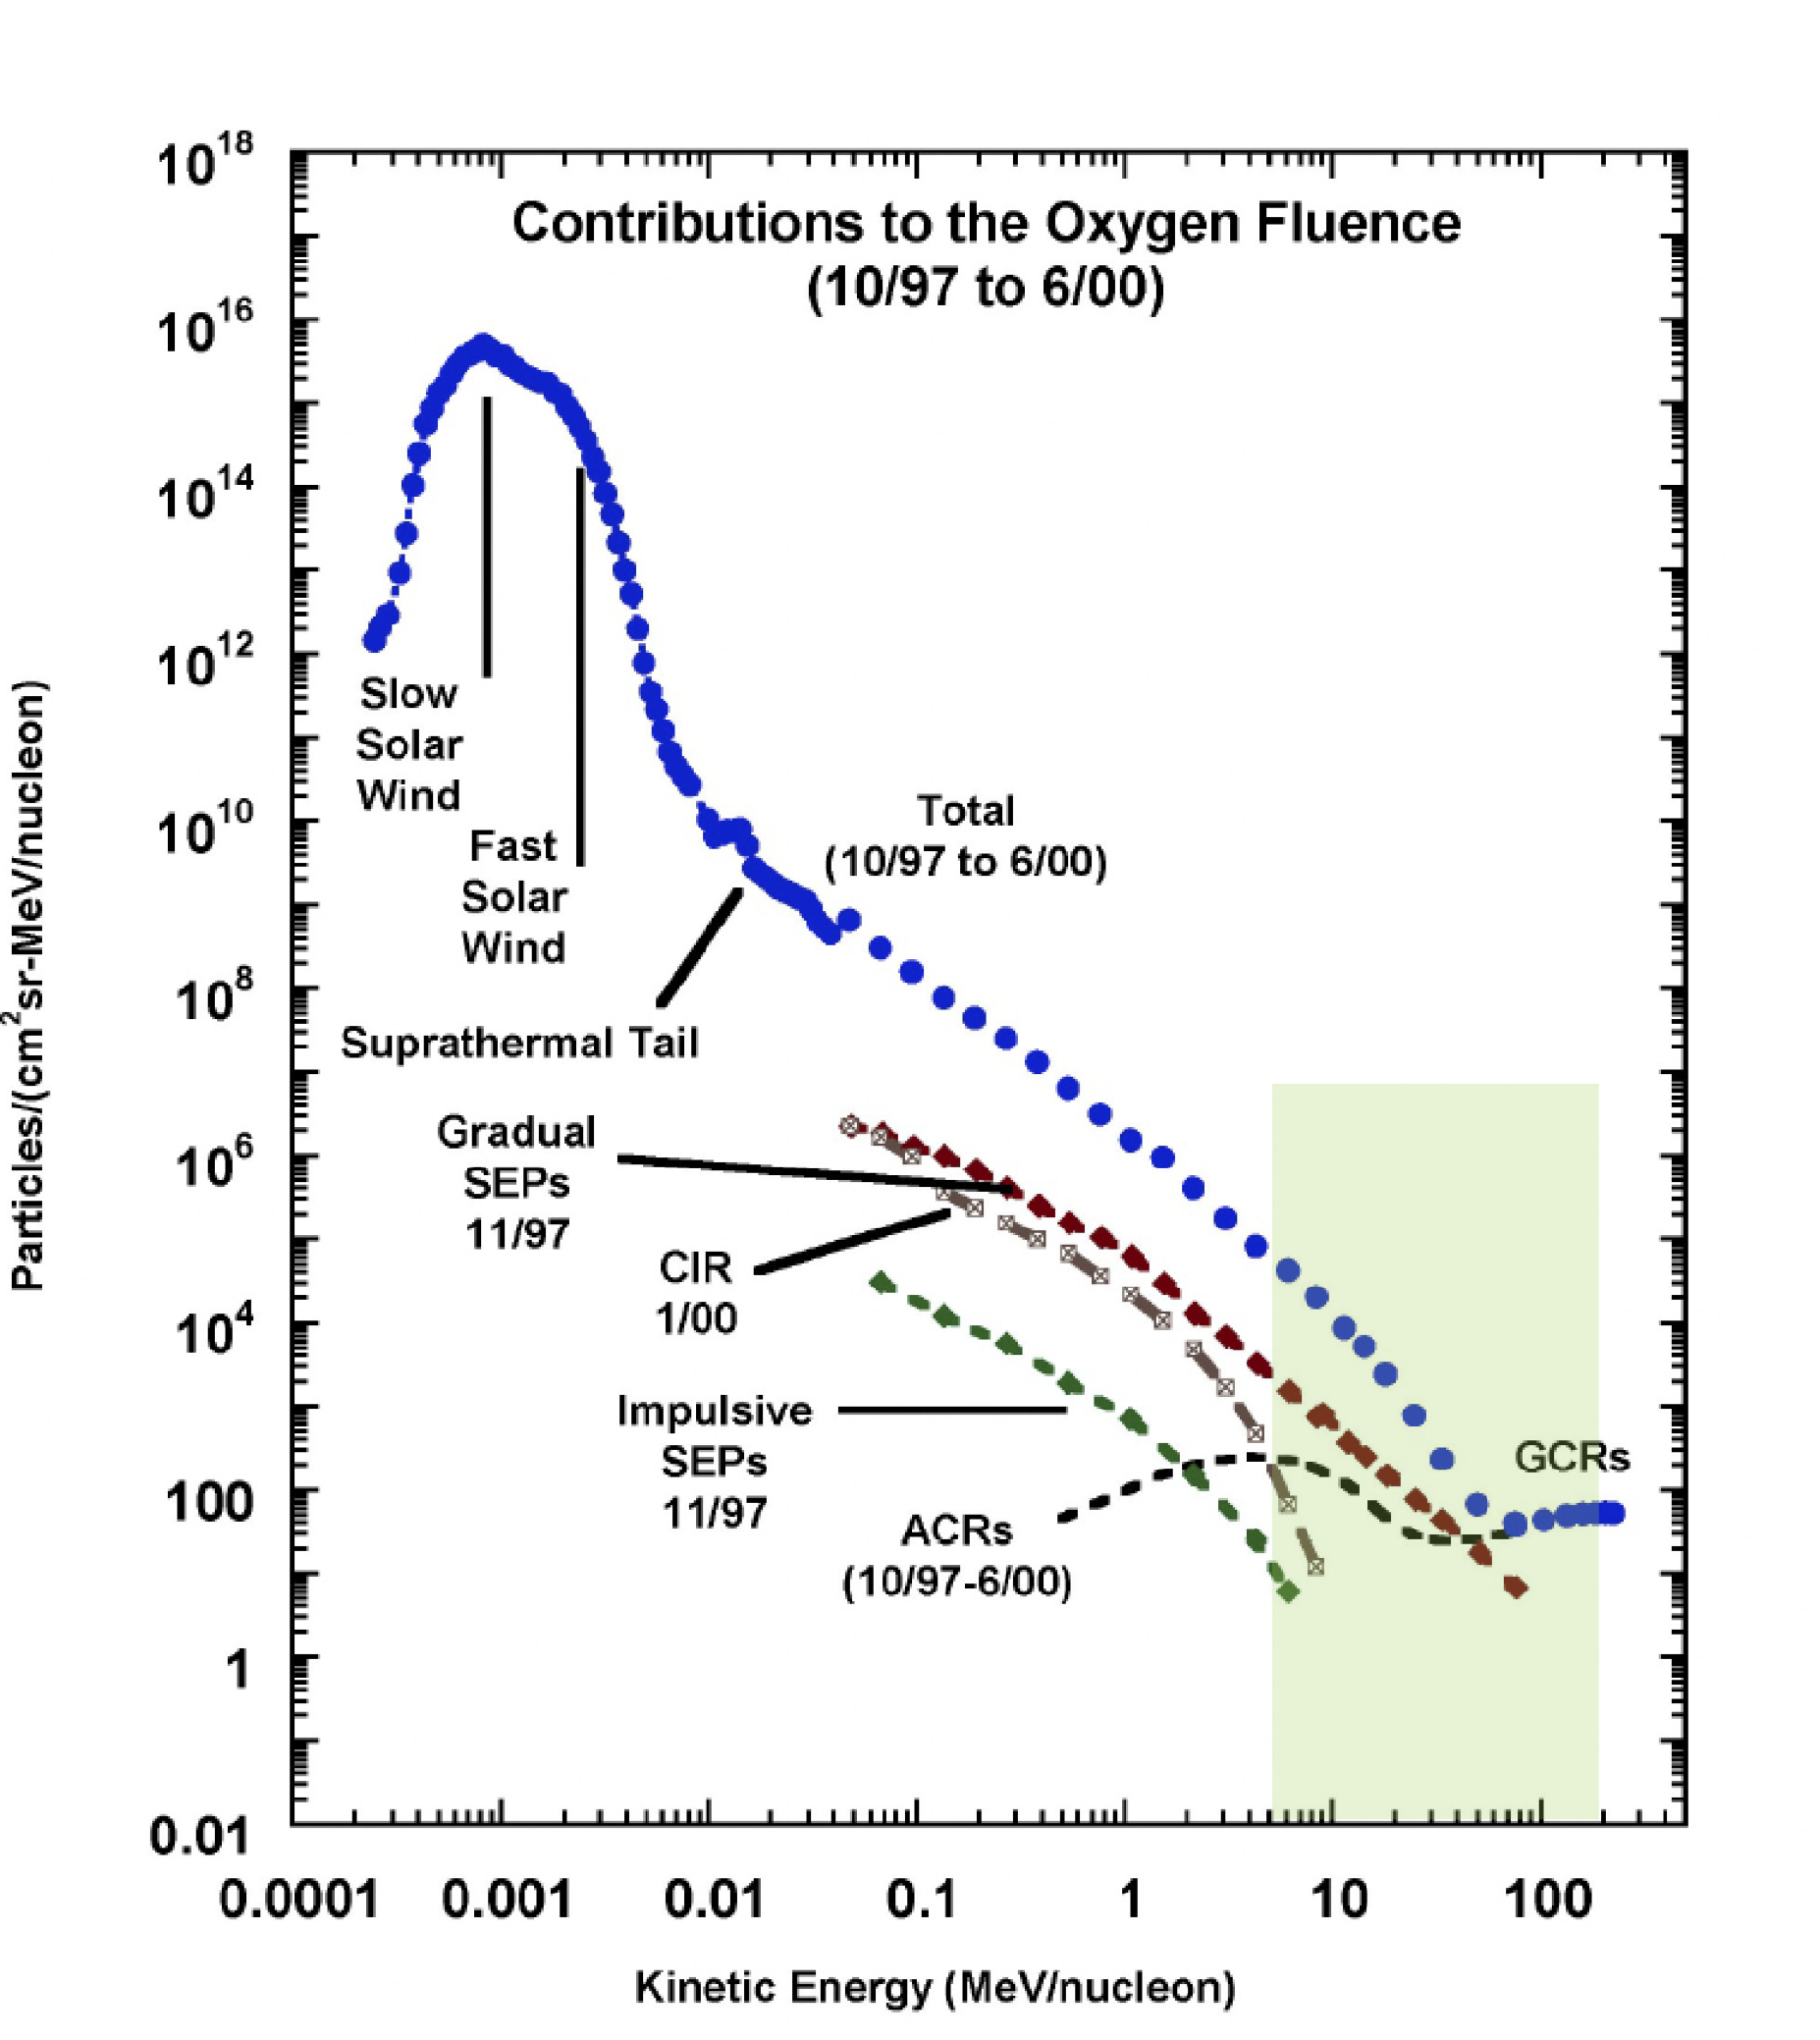
\includegraphics[width = 0.8\textwidth]{images/heliospheric_particle_spectra_color.png}
	\caption[Energy spectra of oxygen ions in the near Earth space]{The typical oxygen spectra in the interplanetary space near the Earth, indicating the contributions of different populations, especially in the energy range between few MeV\/nuc and few hundreds MeV\/nuc, where \acs{SEP}, \acs{ACR} and \acs{GCR} both exist. The spectra of other particles species for instance, helium and proton, have the similar shape but different flux level on corresponding energy region. The figure is adapted from \citep{Mewaldt-2001}}
	\label{Fig:Oxygen_spectra_heliosphere}
\end{figure}

Heliosphere is a vast, bubble-like region in the space that is surrounding the Sun. This region is moving in the \ac{ISM} with a speed of 25 km/s [citation]. Such a cavity is created by the sun and governd by its magnetic field and solar wind; a huge amount of plasmas of various particle populations fill this space. The particle populations could be identified from Fig.\ref{Fig:Oxygen_spectra_heliosphere} which is adapted from the measurements by \citet{Mewaldt-2001}. Based on the accumulated measurement of oxygen by \ac{ACE} between 1997 and 2000, the fluence oxygen spectrum which span over the energy range of more than 7 orders of magnitude from keV/nuc to GeV/nuc show clearly the lower energy particles including solar solar wind, fast solar wind,suprathermal tail, and high energy particles consist of \ac{SEP}, \ac{CIR}, \ac{ACR}, and the extremely high energy \ac{GCR}. 
Among them \acs{GCR} are from very distant source out of solar system, \acs{ACR} source are around the boundary of heliosphere, and the remain energetic particles are the parrticle accelerated and generated inside of the heliosphere at the locations including solar, interplanetary space and even the several planets of solar system for instance Jupiter.

Solar wind is a charged particles stream, also called plasma, released from the solar corona. Such a group of plasam consists of mainly protons and electrons that continously flow outward and expend to about $\sim$ 100 au (differ in the directions). The typical energy range of the solar wind is between 0.5 keV and 10 keV. Depending on the locations on the sun that produces the solar wind, the speed and density of solar wind might be different. For instance the fast solar wind with a typical speed between 500 and 800 kilemeters per second emits from the coronal holes which are funnel-like regions of open field lines in the magnetic field and usually appear in the north and south pole of sun. Therefore, the fast solar dominate the high latitude regions. While the slow solar wind is observed to have a velocity of about 300 - 500 kilometers per second and is believed to originate from the streamer belt along the equatorial belt. The slow solar wind is more likely to be observed in the low latitude regions.

%plasma embedding with magnetic field

Suprathermal particles are charged ions and electrons that move about two to hundreds times faster than the solar wind. In the spectrum shown in Fig.\ref{Fig:Oxygen_spectra_heliosphere}, the suprathermal particles are beyond the tails of the fast solar wind and are the dominate particles between few keV to hundreds of keV. The source of suprathermal particle might be the acceleration of solar wind and the remanent of the previous solar eruptions and \ac{SEP} events. Those particles play am important role in contributing seed particles for the \acl{SEP}	events.

Above the energy suprathermal particle are the energy range that we are interested in this thesis, especially the energy range between 10 MeV/nuc and few hundred MeV/nuc where the dominated particles are solar energetic particles (not limited to this energy range), anomalous cosmic rays (up to $\sim$ 100 MeV/nuc) and lower energy galactic cosmic rays. The new measurements in this study are from this energy range.

The \acl{SEP} are the high energetic particles with energy of few keV up to $\sim$ GeV oriented from the sun and accelerated during the solar activities like solar flare and \ac{CME} driven shocks. \acs{SEP} events are recurring, short term, but intensive. Different type of \acs{SEP} events persist different time scales, various from less than days to few days. Such high energy particles are one of the major threats in the space.
%also particle from solar, accelerated by different mechanism. The enery range of \ac{SEP} are quite broad, especially depending the on where the measurement carried on. Recently \ac{SOLO} and \ac{PSP} frequently measure the hundreds keV \ac{SEP}.

\acs{ACR} are the high energy interstellar pick-up ions [citaion] which are ionized neutral interstellar atoms generated by solar UV radiation after they move cross the boundary and enter the heliosphere. Those ionizing particle are then carried by the expanding solar wind to the outer boundary of helioesphere, where they are accelerated by the termination shock and then propagate inwards. The typcial species that have been observed are proton, helium, oxygen, nitrogen, iron, neon, etc. [citaion]

\ac{GCR} are the fully ionized particles that is accelerated at the so-called supernova remnants \cite{Blasi2013AARv2013} which are outside of the solar system and bombard Earth in a slowly varying and constant way. The complete GCR spectrum cover the energy from typical 1MeV \citet{Potgieter2013LRSP} to ZeV which is way beyond the energy range in Fig.~\ref{Fig:Oxygen_spectra_heliosphere}. The \acs{GCR} is comprised of about 89\% of hydrogen, 10\% of helium, 1\% of heavioer ions as well as electron, positron and antiprotons. 

After entering the heliosphere, the transport of both cosmic rays are controled by the \ac{HMF}, hence \ac{ACR} and \ac{GCR}'s temporal variaton is highly related with the solar activities and the so-called solar modulation, which are periodcally change in 11 and 22 year periods. 


\section{Solar energetic particles}

\subsection{Two types of SEPs}


The first observation of \ac{SEP} events was made back to a magnetic storm on March 1, 1942 \citep{lange1942note,forbush1942further}, during which three unusual increase in the cosmic-ray intensity was observed on ground-based ionization chambers and the neutron monitors and appeared simultanously with the solar flare eruptio. Later, \citep{Forbush1946} attributed such increases to the charged particles oriented from the sun with sufficient energy to penetrate the Earth's atmosphere. Now we have known that this is the so-called \ac{GLE}, one type of the most hazard energetic particles in the space which is actually the \ac{SEP} of more than 433 MeV/nuc energy, typical more than GeV. \citep{meyer1956solar,Shea2012SSRv,gopalswamy2013first,thakur2014ground, Reames2013}.

It is commonly believed that the generation of \acp{SEP} are highly related to the solar flare during first few decades after the discovery of \ac{SEP} because they generally appeared simultanously. This is so-called "solar flare myth" as discussed in \citep{gosling1993the}. At the same time, the important role of CME and its driven shocks in the generation of \ac{SEP} was largely underestimated, though a quite lot researches on the characters of such \acp{SEP} like the duration, longitudinal distribution, the abundance of the typical elements and their association with radio burst had indicated the existence of two types of distinct events - impulsive and gradual \ac{SEP} events \citep{kahler1978prompt,kahler1984associations,cliver1982injection,cane1986two, reames1988ApJ}.
Currently, the scientists have generated such a classic two-class picture (See,\ref{Fig:two_type_SEP},\ref{Tab:Two_type_SEP}) which has been widely accepted by the science community \citep{kallenrode2003current, reames2013two,Desai_Diacalone2016LRSP, Reames2021LNP}. Both acceleration mechanisam and the source locations are different for two type of \ac{SEP}.


Fig.~\ref{Fig:two_type_SEP} illustrate the current scenario of gradual (left) and impulsive (right) \acp{SEP}.
The gradual events are diffusively accelerated by the CME-driven coronal and interplanetary (IP) shocks. Generally, a complete gradual \ac{SEP} event that connects to the shock nose usually consists of an sharp increase phase as the start, a long lasting plateau and a flux peak at lower energy which indicates the arrival of \ac{CME} at the detector. The whole process might persist from one day to several days. Gradual \ac{SEP} is always accompanied by the type II radio burst, which is a broad and slow shift struture in the radio dynamic spectrum. Type II radio burst is considered as a signature of \ac{CME} and track of the propagation of \ac{CME} from the sun to 1 au. Shocks mainly accelerate protons and heavy ions, but not the electrons with the same efficiency, causing the large discrepancy of ratio of electron to proton between two types of \acp{SEP}.
Besides, the gradual \ac{SEP} spread widely in the IP since \ac{CME} has broader longitude extend and can be measured by multiple detectors even if they are far away from each other. In the next section, we will discuss more about the widespread event. The appearance frequency of gradual \ac{SEP} during the solar maximum is about $\sim 100$ per year

While the solar flare which erupts from the solar active region is considered as the souce of the impulsive \ac{SEP} event. The fierce magnetic reconnections during the flare eruption can accelerate particles, especially electons, to high energies up to hundred MeV. Therefore, the electrons are the dominant particles. Besides, in this senario, the particles escape from the open magnetic field and arrive at the Earth along the spiral magnetic field (Parker spiral, \citep{Parker-1958}) that is shaped by the expanding solar wind. From the Earth's point of view, the impulsive \acp{SEP} are typically located in a narrow region in the west hemisphere of sun. Type III radio burst usually appear with impulsive event, but no \ac{CME}
The appearance frequency of impulsive \ac{SEP} during the solar maximum is about $\sim 10^3$ per year. The typical duration of impulsive \ac{SEP} is less than days.
It is worth noting that, \citep{cane2003two} found that some intensive \ac{SEP} have two components related both flare and shocks. Such events are called mixed events that have flare particles as seed population and later those particles are reaccelerated by the shocks. [Might find a paper and confirm the statements]

In Tab.~\ref{Tab:Two_type_SEP}, we summarized the general properties of the two types of \ac{SEP} events.

\begin{figure}
	\centering
	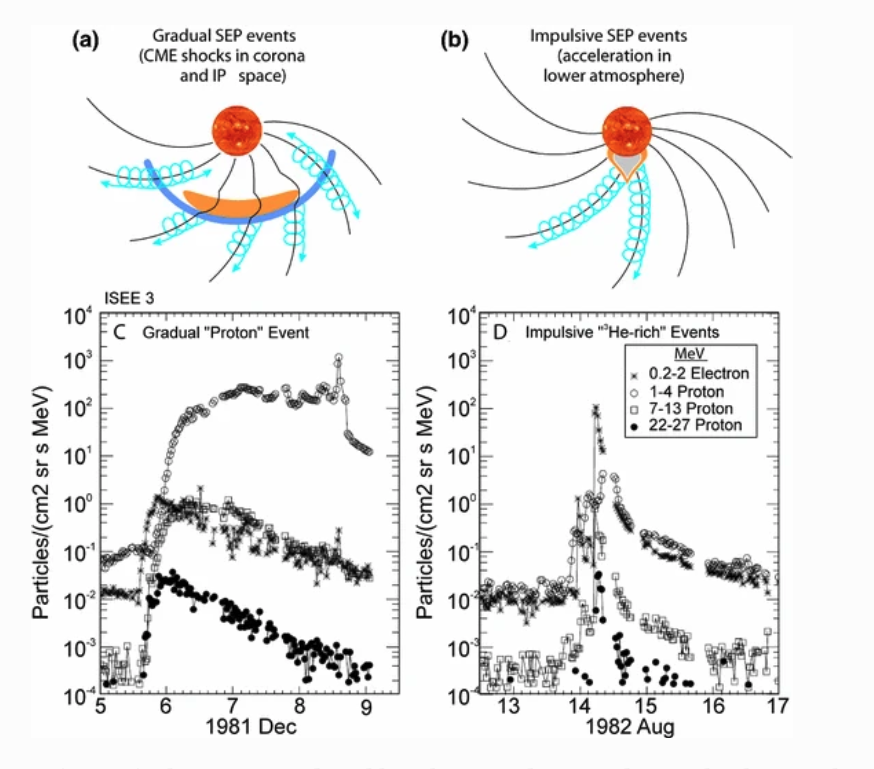
\includegraphics[width = 0.75\textwidth]{images/SEP_two_type.png}
	\caption[Two type of Solar energetic particle (SEP) event]{Two class of SEP events is presented. (a) The gradual SEP events that are associated with the CME drivens shocks in the coronal or in the interplanetary space and the particles populate the interplanetary magnetic field (IMF) lines over a wide range of longitudes. (b) The impulsive SEP event that is associated with the solar flares and the particles only populate a limited range of the open IMF lines that are well-connected to the flare site. Plots (c) and (d) are the corresonpding typical proton and electron time profile of the large gradual and small impulsive SEP events. The figure is reproduced from \citet{Desai_Diacalone2016LRSP}.}
	\label{Fig:two_type_SEP}
\end{figure}


\begin{table}{!h}
	\centering
	\caption[Two classes of SEP events]{Two-class paradigm of \ac{SEP} event, adapted from \citet{kallenrode2003current,	Desai_Diacalone2016LRSP, Wang2009}.}
	\begin{tabular}{c|c|c}
		\hline
		\hline
		Property 	& Gradual \ac{SEP} 	& Impulsive \ac{SEP} \\
					& (Large \ac{SEP})	& (Electron/$^3$He-rich \ac{SEP}) \\
		\hline
		Dominant particle	& proton	& electrons \\
		Electron/proton ration &  50 - 100 &  $10^2 - 10^4$  \\
		$^3$He/$^4$He ratio	& 4$\times$ 10$^-4$ & 1 \\
		Fe/O			& $\sim$ 0.1			& $\sim$ 1	 \\
		H/He		 	& $\sim$ 100			& $\sim$ 10 \\
		Q$_{Fe}$		& $\sim$ 14 			& $\sim$ 20 \\
		Duration		& $\sim$ Days			& $\sim$ hours \\
		Longitude cone	& > 100 $^\circ$		& < 30$^\circ$ \\
		Seed particles	& Ambient Corona or Solar wind & Heated corona \\
		Radio type		& Type II/IV	& Type III \\
		X-ray duration	& $\sim$ hours	& $\sim$ minutes - 1h \\
		CME association	& Fast/halo CME	& No	\\
		Frequency(at 	& $\sim$ 10	& $\sim$ 1000 \\
		solar maximum)	& 	& 	\\
		\hline
	\end{tabular}
	\label{Tab:Two_type_SEP}
\end{table}


\subsection{Wide-spread SEP and Multiple instruments observation}


\begin{figure}
	\centering
	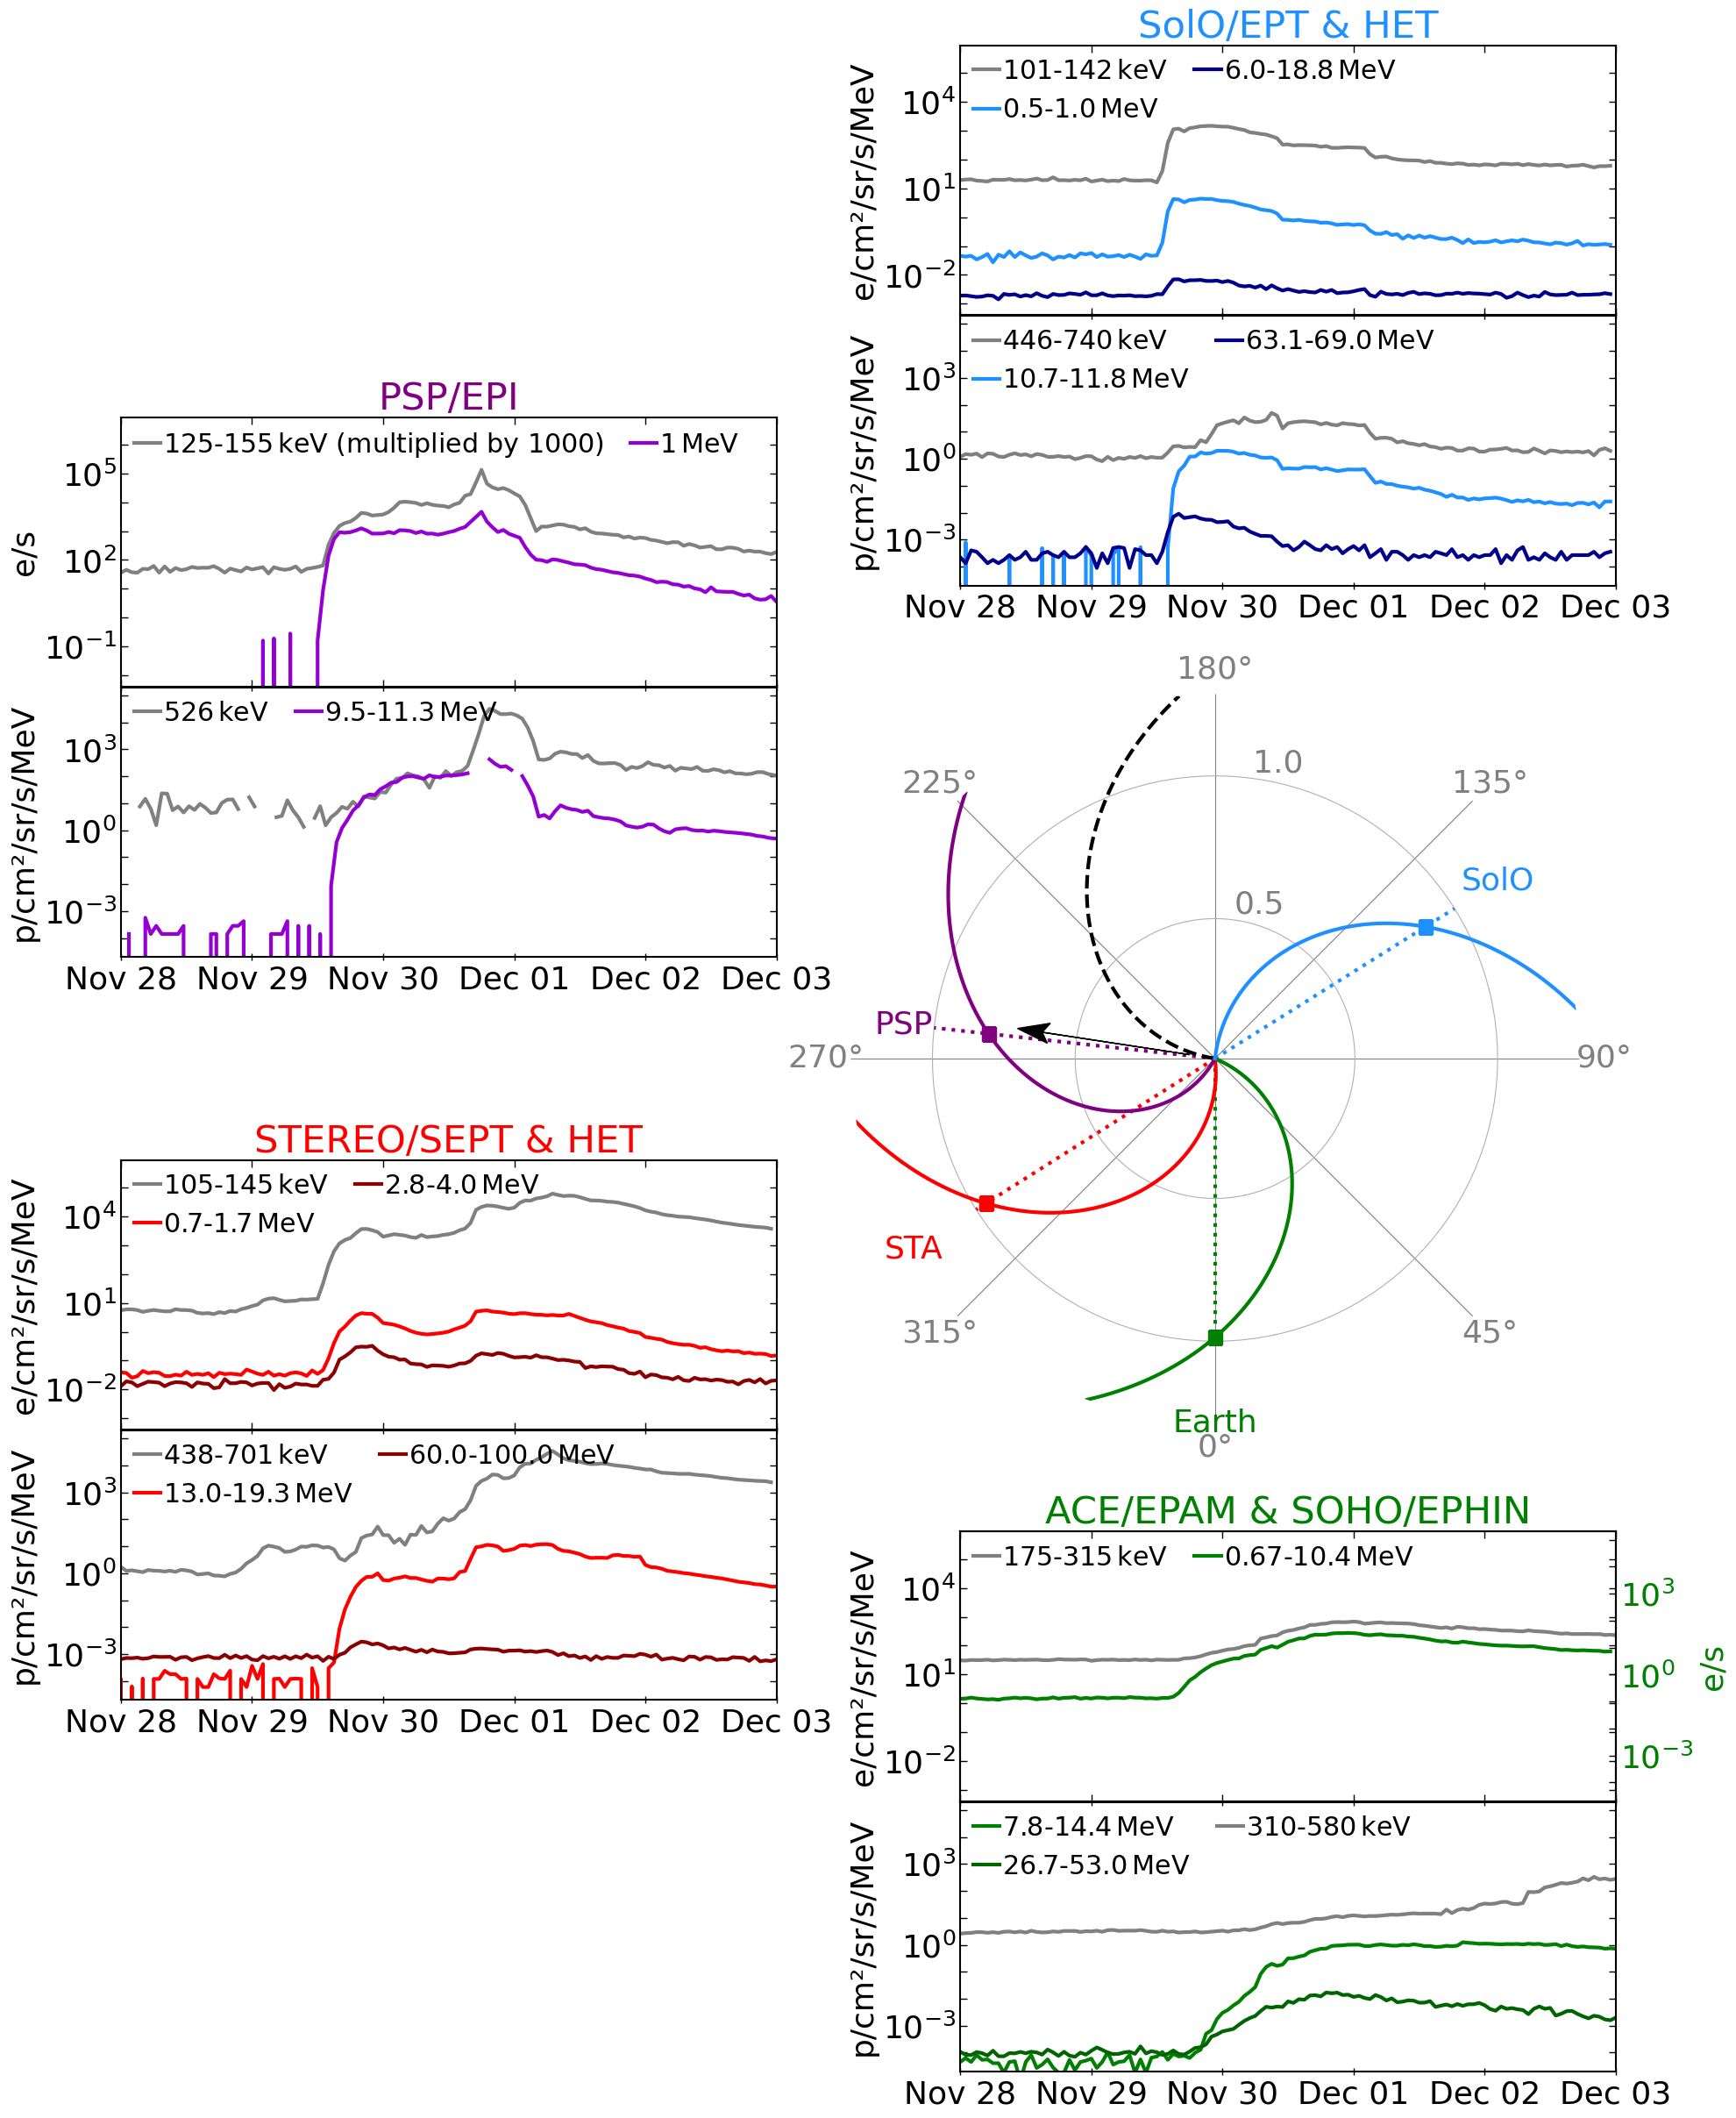
\includegraphics[width = 0.7\textwidth]{images/2020-11-29_overview_plot.png}
	\caption{The first wide-spread \acl{SEP} event on Nov 29, 2020. The figure is from \citep{Kollhoff-2021}}
	\label{Fig:SEP_widespread}
\end{figure}

Due to limited space in the introduction part, we could not go through all aspect 
related to the \ac{SEP} thoroughly which can be refered in the review papers, for instance the remote-sensing observation of SEP like radio, EUV, X-ray and the problem regarding the injection and transport, composition, charge state, anisotropy and spectra evolution can be found in the review papers \citet{reames2013two, Desai_Diacalone2016LRSP, Reames2021LNP}
Instead, in this part we shorlty introduce the wide-spread SEP and the multiple instruments observation of SEP.

Figure \ref{Fig:SEP_widespread} is the first widespread \ac{SEP} of the \ac{SC} 25 observed by \ac{SolO} and simultanously by \ac{PSP}, \ac{STEREO}, \ac{ACE}\/\ac{SOHO} near the Earth on 2020 November 29 \citet{Kollhoff2021AA, Kouloumvakos2022, Palmerio2022}. Both relativisitc electons and higher energy protons with energy >50 MeV were observed. This SEP was associated with an M4.4 class flare accompanied by a \ac{CME}, \ac{EUV} wave, type II/III radio burst. The particles spread over a more than 230$^\circ$ longitude regions at 1 AU. The black arrow in the middle panel indicates the location of the active region and the possible location of the central meridian of the \ac{CME}.  Depending on the magnetic connection between \ac{CME} shock and instrument at different locations, the time profiles of particles are different. For instance, \ac{PSP} and \ac{STEREO} connect closely to the central meridian, hence the intensity profile shape are similar with the \ac{SEP} we showed in Fig.~\ref{Fig:Two_type_SEP}, i.e., abrupt increase plus a peak when the shock reached the s\/c location. While Earth is about 166$^\circ$ away from the active region and connect to the west limb of the source, the intensity of the event slowly increased.
Recently a comprohensive study of the second widespread \ac{SEP} of \ac{SC} 25 occured on 2021 April 17 is carried by \citep{dresing202317}. It was detected over a more than 210$^\circ$ longitudianl region at 6 location including four locations used in the previous event, \ac{Bepi} and Mars from different radial distance, though the Mars observation only provide a observational contrain. \citep{dresing202317} argue that the distinct SEP injections cover a wide range of longitudes might be responsible for this widespread SEP event.

As indicated from two examples, the wide spread \ac{SEP} event is type of event that particles can spread over a large range of longitude (\> 200$^\circ$), and persist for few days, somesome

One of the most important question of SEP is how the energetic particle spread the heliosphere. The possible mechanism of the large spread SEPs including Magnetic connection to an expanding coronal and IP shock, Coronal transport, multiple particle injections, EUV waves, cross-field diffusion, meandering magnetic field lines, particle transport to remote longitudes by large-scale magnetic loops.

%In the above two example, we have already use multiple instrument to study the \ac{SEP} events. While the history of multiple observation dates back to 

%Nowadays, more and more space-born telescopes have been developed and launched to study the center of our heliosphere and moniter the variation of the plasma environment.  
%Study both in-situ and remote.
%Now - \ac{SOLO} \ac{PSP} and \ac{Bepi},  Mars, STEREO missson, helios mission, new mission from China, \citet{Wang2020Solarring,}India

%A numerous observation and simulation studies have been carried on in the past few decade since the discovery of SEP back to 1950s. The major questions of SEP focus on the origin, acceleration and transport of those high energy particles.\citep{Desai_Diacalone2016LRSP}, which is also the goal of recently two missions \ac{PSP} and \ac{SolO}. 




%=========================================

\section{Galactic cosmic rays}

\begin{figure}
	\centering
	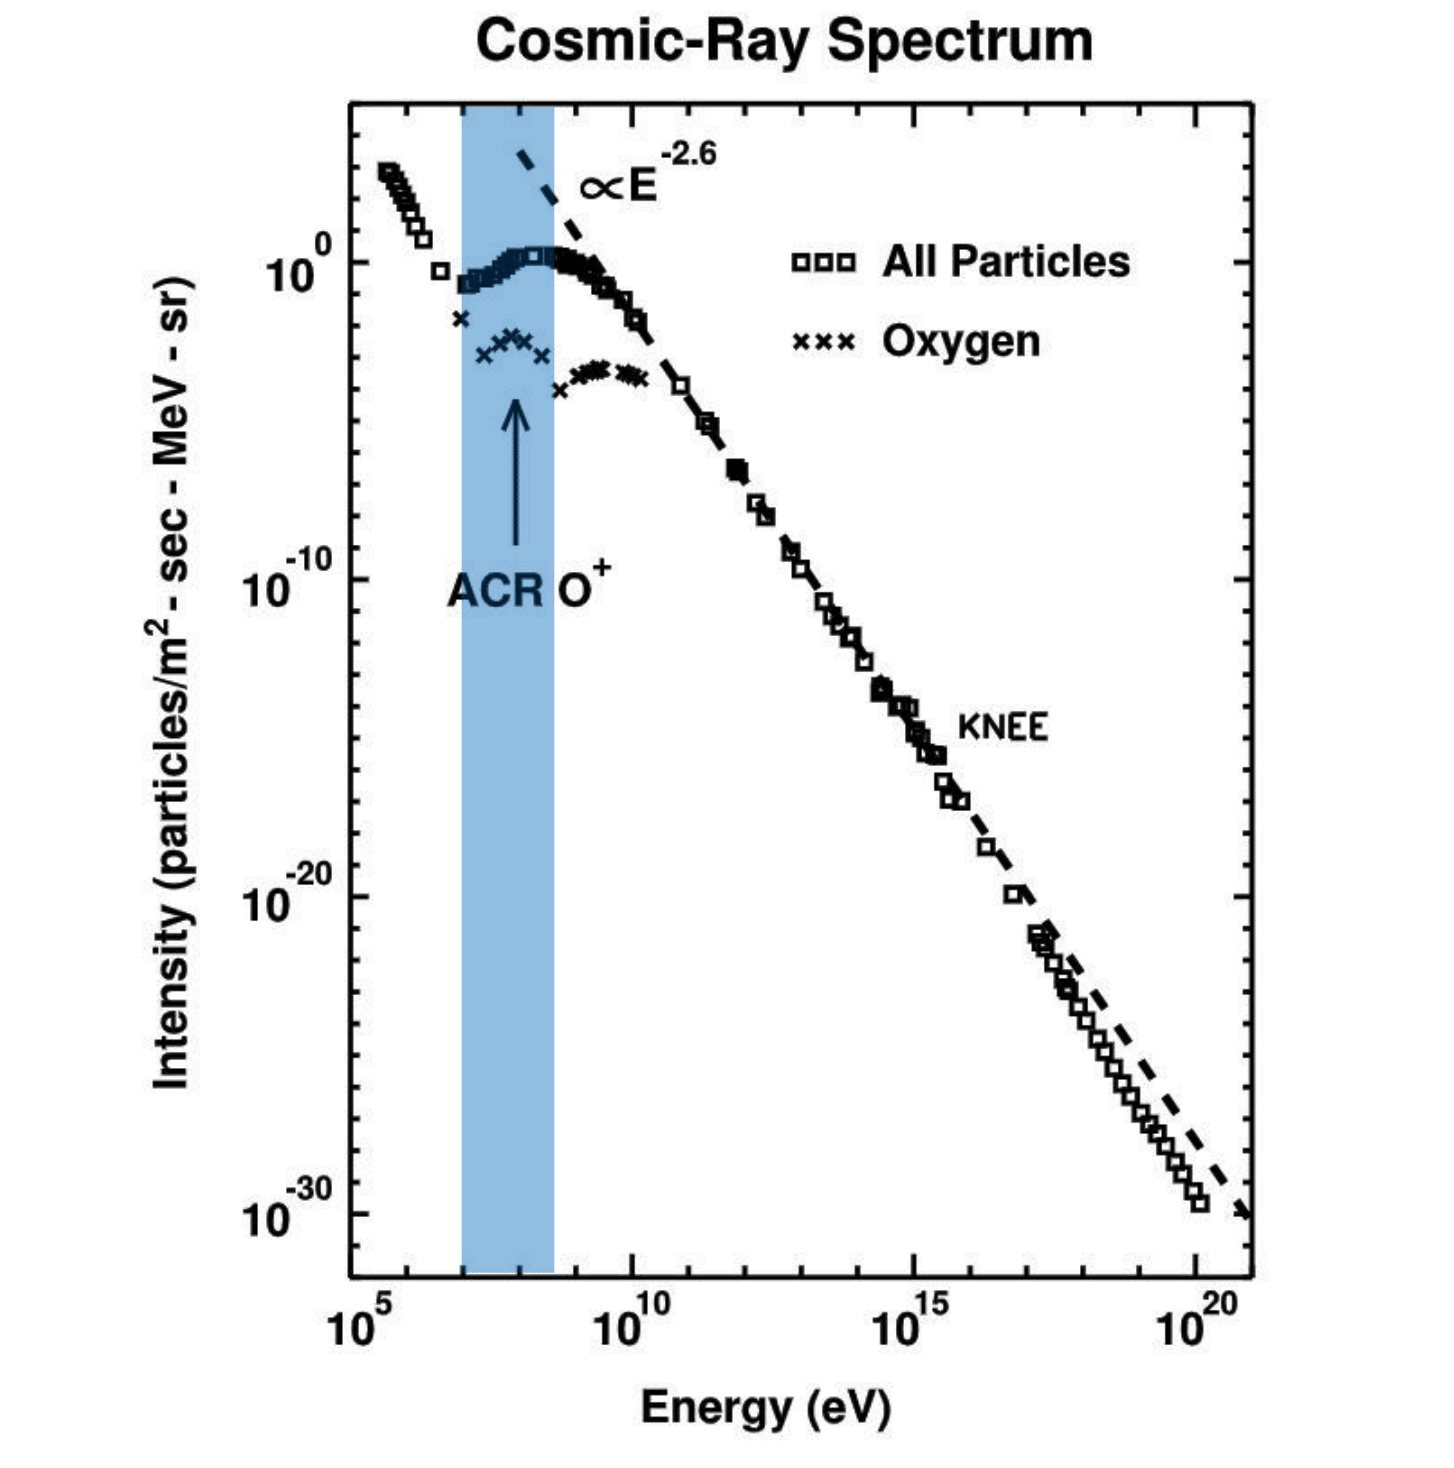
\includegraphics[width = 0.7\textwidth]{images/gcr_spectra_shadow.png}
	
	\caption[The cosmic ray spectra of all particles at 1 au]{The cosmic ray spectra of all particles and ACR oxygens observed at 1 au. This figure is from Giacalone 2021, 2012, and originally from Jokipii 1990.
	The spectrum is plotted in more than 15 orders of magnitude on the energy scale and about 30 orders of magnitude on the intensity scale, extend the high energy end of Fig.\ref{Fig:Oxygen_spectra_heliosphere}.}
	\label{Fig:Oxygen_spectra_cosmic_ray}
\end{figure}
%\url{https://timeline.web.cern.ch/victor-hess-discovers-cosmic-rays-0}
The first discovery of the galactic cosmic rays was made by the Victor Hess in 1912 when he carried on a ballon experiement. The initial purpose of the experiement was to find the source of ionizing radiation in Earth's atmosphere using the electroscope. However, as the ballon climb-up during the experiment, he found that ionization rate measured in the electroscope showed less signicant decrease than anticipated. Such a discrepancy was attributed to the existence of the cosmic rays which increase the radiation in the atmoshphere.

In figure \ref{Fig:Oxygen_spectra_cosmic_ray}, the full spectrum of the all cosmic particles observed at 1 AU which includes both the \ac{ACR} and \ac{GCR} components is shown. The \acs{GCR} are indicated as empty squares. In the right half of the spectra with energy above 1 GeV, the spectrum could be simply fitted by power a law spectrum with index of about -2.6. The knee of GCR spectra are around [] energy and reflect what mechanism[citation]. The lower energy spectrum is shown as a "turn over" below 1 GeV which are more complicated and could not be fitted by a signel power law. 

\acs{GCR} consist of multiple energetic particle species span a wide range of energy, which are mostly dominated by the proton, about 89\%  and the remains are shared by 10\% helium and a small portal of heavier ions (1\%), electron, positron and antiproton. 
It is believed that \acs{GCR} are mainly originated from the supernova remanent very far from the sun[citation] and obtain the energy from the shock waves which is genereated from the explosion of supernova. When the shock wave travel through the surrounding interstellar gas, the kinetic energy of shock are tranfer to the  (neutral gas?) by the (Fermi-acceleration, ciataion and the acceleration process), Utilimatly, the energetic particle with energy up to 10$^12$ eV are created.
After a long travel, \acp{GCR} arrived the local bubble controled by the sun and its magnetic field. Before entering the heliosphere,  the particles are isotropic distributed in space and nearly constant  in time. Because cosmic rays are fully charged, they are deflected by the magnetic field when they propagation in the interstellar space after speeding up. The directions of those particle are normalized by the strong magnetic field. Hence when they arrived at the local bubble of solar system, we obtained an nearly isotropic and constant intensity profile [citaion of the LSTM,]

To model the solar modulation on the particle transportation of GCR spectra, an input particle spectra need to be specifield, which is the so-call LSTM [ citaion of LSTM]. LSTM is the modulation boundary and will be modulatined as the change of the position, energy, and time after those particle diffusion into the heliosphere. Such a spectra have been observed by the voyeger after then cross the boundary of solar system and enter the interstellar medium.

% As shown in the Fig.\ref{Fig:Oxygen_spectra_heliosphere}, the dominated energy of \acs{GCR} is above 100MeV/nuc.  
% ---- To do
% [Describe the GCR spectra]
% Below that, the other component are more common than GCR and it is hard to seperated those particles.
%  ---
%A paragraph of local intersteallar spectra ?

After enter the heliosphere, those high energetic particle are modulated the solar wind and its embedding magnetic field  which changes in a 11 year or 22 year period, which is so-called solar cycle.
The relavant process of the solar modulations could be described by a basic transport equation (TPE) which is first derived by Parker (1965). The same equations was also derived by Gleeson and Axford (1967) in the more rigorous ways. This equation is based on the motion of charged and particle in the high frequently changed magnetic field and averages over the pitch angle of particle moving in the magnetic field. The precondition of this equation is the reasonable assumption of the isotropically distributed GCRs. The TPE give the phase-space distribution function, $f$ as the function of positions, time and momentum magnetitude. In Potgieter (2013), the helispheric TPE, based on Parker (1965) is rewritten in the following form:

	\begin{equation}
		\underbrace{\frac{\partial f}{\partial t}}_{a} = - ( \underbrace{\boldsymbol{V}}_{b} + \underbrace{\langle v_d \rangle }_{b}) \cdot \nabla f + \underbrace{\nabla \cdot (\boldsymbol{K_s \cdot \nabla f})}_{d} + \underbrace{\frac{1}{3}(\nabla \cdot \boldsymbol{V}) \frac{\partial f}{\partial ln P}}_{d}
		\label{Eq:Transportation_equation}
	\end{equation}

where $f(r, P, t)$ is the cosmic ray distribution as the function of the time t, particle rigidity P and 3-dimension position in the space. Compared with the $\sim$ 11 years solar cycle, the periodcally solar rotation ($\sim$ 27 days) and  the time of the solar wind traveling to the edge of helipshere ($\sim$ 1 years) are short-term variation and can be neglected. Hence the steady-state solution with  $\frac{\partial f}{\partial t} = 0$ (part a of Eq.\ref{Eq:Transportation_equation}) is a reasonable assumption and also considered. Terms in the right parts include four effects that are used to describe the variation of the cosmic rays: (b) convection due to the solar wind velocity $\boldsymbol{V}$; (c) drift effects caused by the gradient and curvature of the large-scale \ac{HMF}, which is estimated by a 3D Archimedean spiral \citet{Parker-1958}, $\langle v_d \rangle$ represents the averaged drift velocity; (d) diffusion effects caused by the turbulent mangetic field, with the $\boldsymbol{K}_s$ the symmetrical diffusion tenser; (e)adiabatic energy change and deceleration due to the expansion of the solar wind. 

Since TPE is a high non-linear partial differential equation, only a simplified solution of the GCR spectra is derived which is called the Force-field Solution (FFS). The FFS was first derived by Gleeson and Axford [1967, 1968b], which simply depend on the kinetic energy T of particles and the solar modu. Later, a reasonable GCR spectra of the particle with energy above 150 MeV were given by Gleeson and Urch 1973.
With the development of computer technque and numerical studies, simulation are becoming more and more important in studying the tranporation and solar modulation of the cosmic rays. [Jokippi and Kopriva 1979, Le Roux and Potgieter 1995, Manuel et al 2011, and Potgieter 2013, Vos \& Potgieter 2015, 2016; Boschini et al. 2019;
Corti et al. 2019; Shen et al. 2019 \url{https://iopscience.iop.org/article/10.3847/2041-8213/acbea7/pdf}]. 
Commonly used model like BON14, 2020, CREME 96 and HELMOD with the solar modulation and sunspot numbers as input could reproduce the GCR intemnsity and spectra which are consistent with the measurements from \ac{ACE} in 1 AU and Voyager probes in the different regions of helisophere [Boschini et al 2019- Model]

\begin{figure}[htbp]
	\centering
	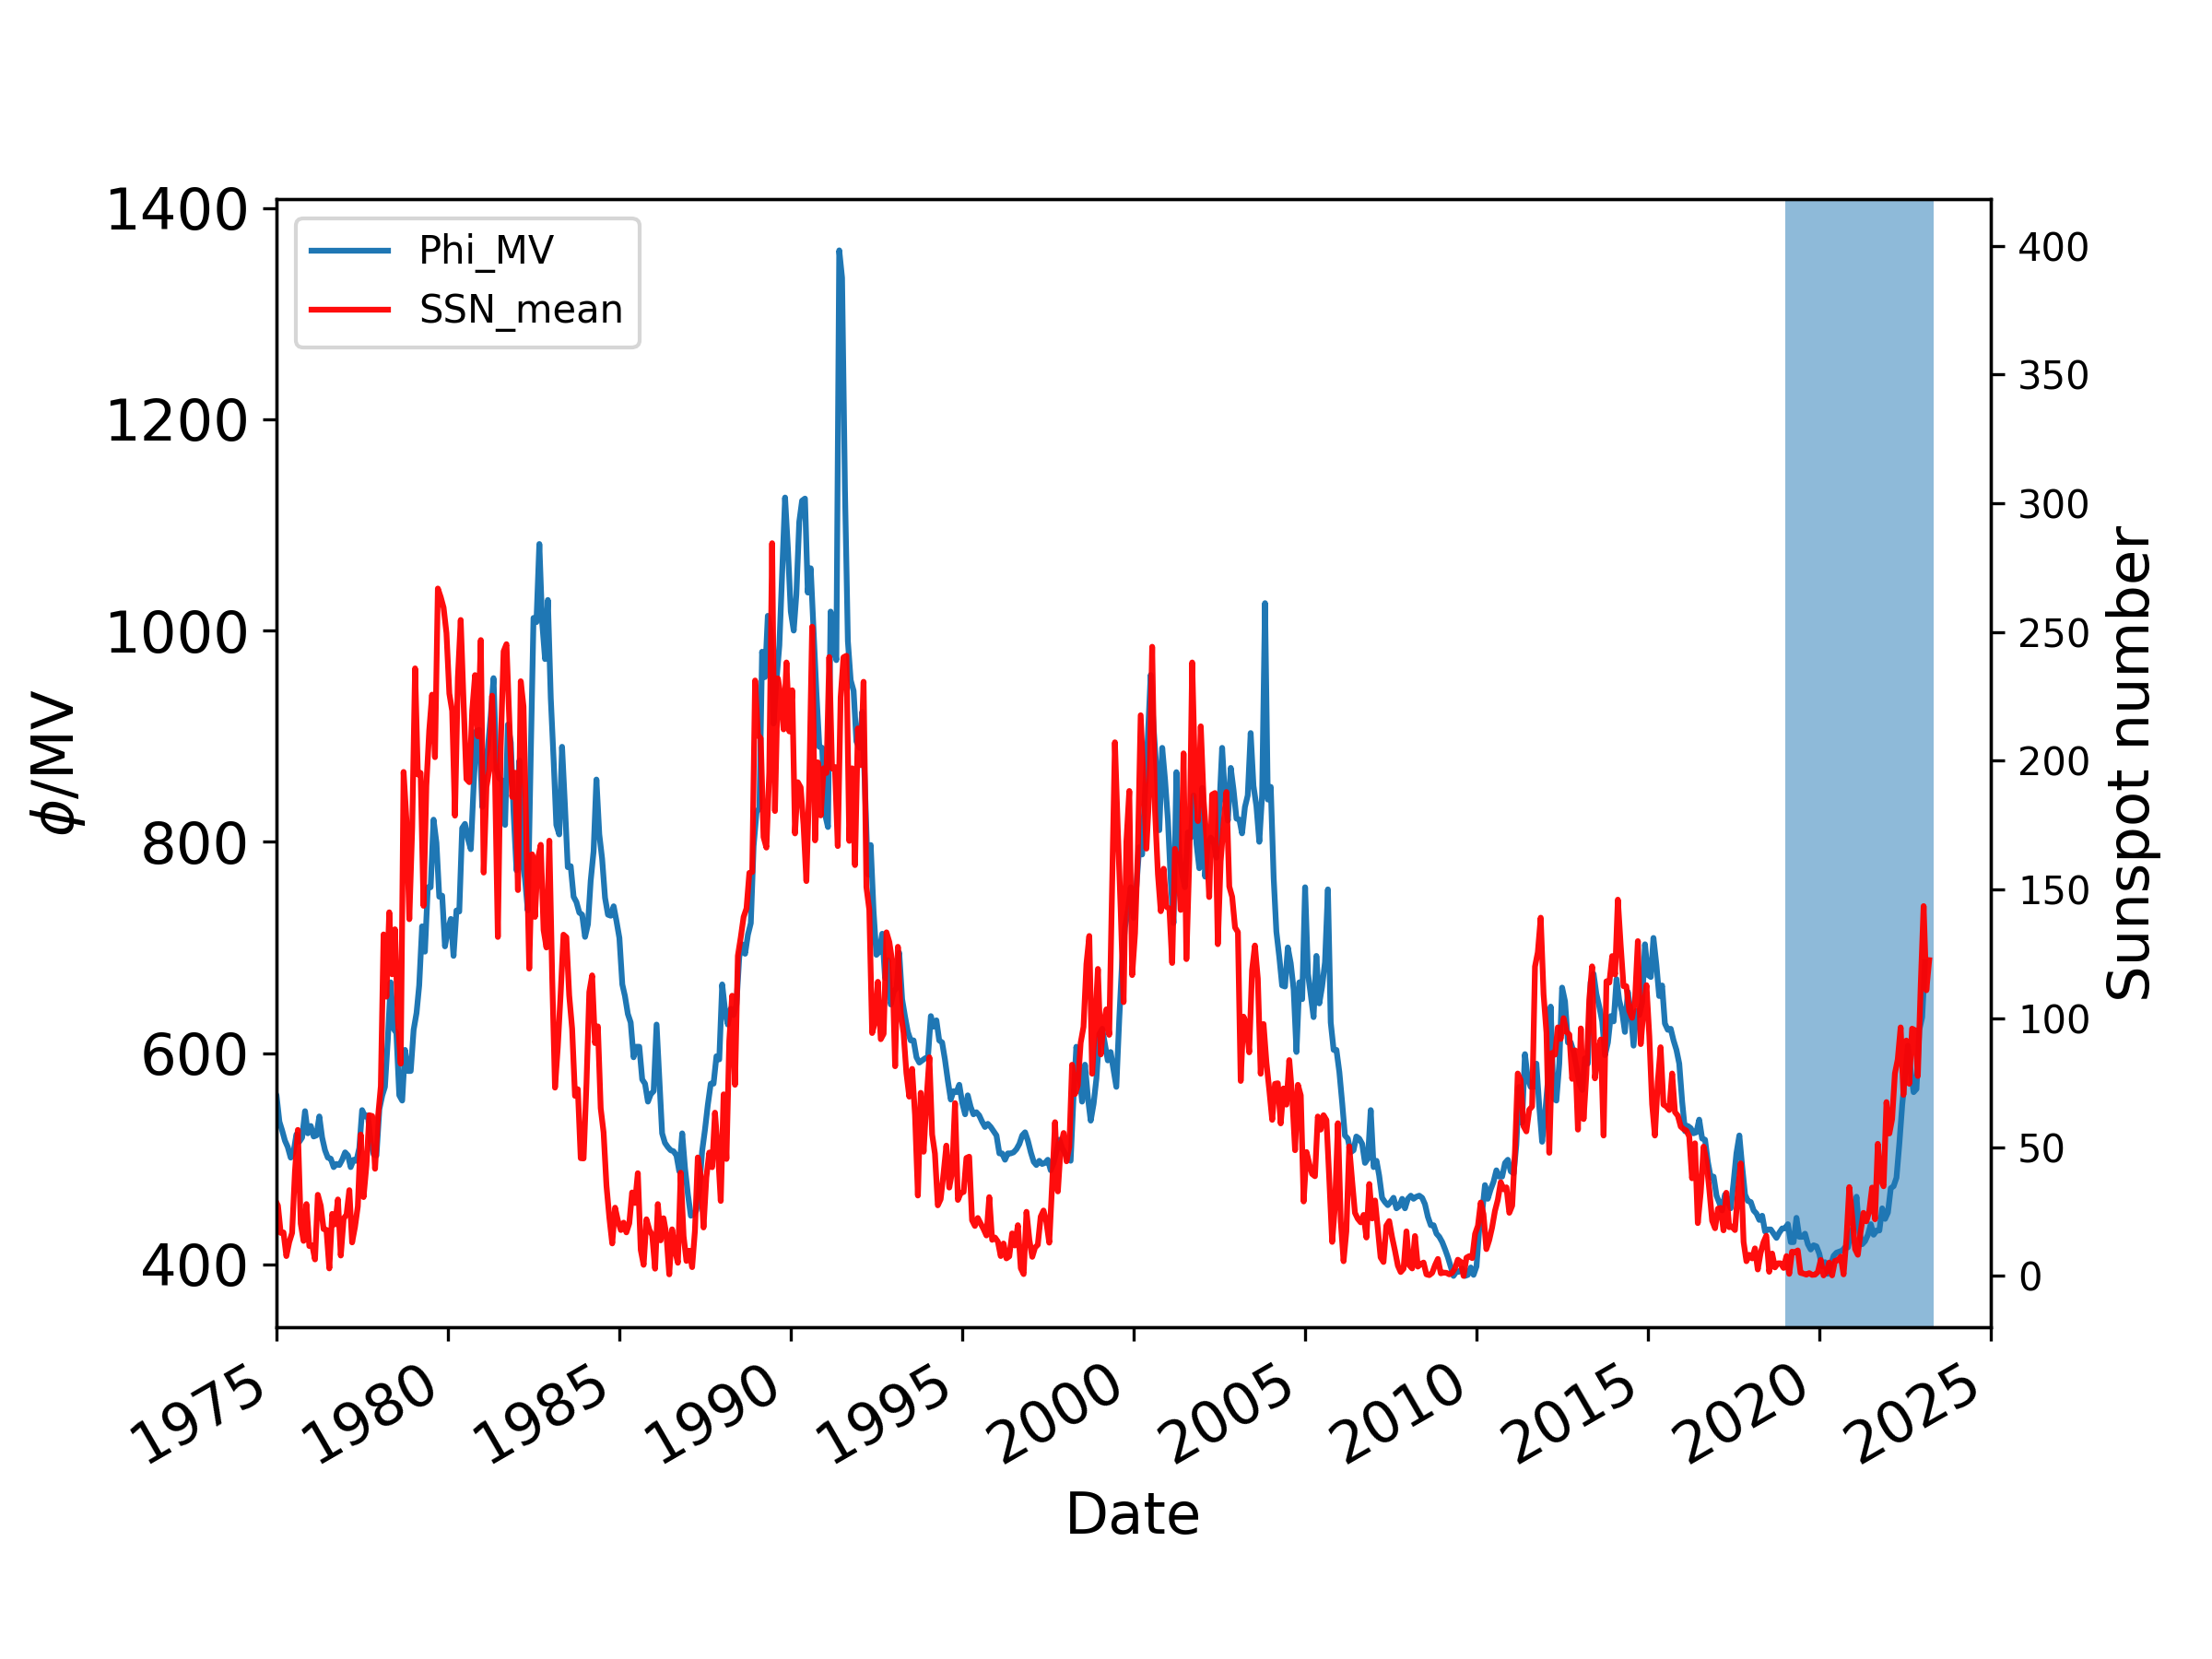
\includegraphics[width = 0.9\textwidth]{images/Solar_modulation.png}
	\caption[Sunspot number and Neutron monitor count data]{Oulu neutron monitor count rate downlowded from \ac{NMDB} \footnotemark[1] measured by Sodankyla Geophysical Observatory of the University of Oulu, Finland and the monthly averaged sunspot number from Solar Influences Data analysis Center (SIDC) \footnotemark[2], Royal Observatory of Belgium, Brussels. The period that we are interested in is marked by the shadow region.}
	\label{Fig:Solar_modulation}
\end{figure}
\footnotetext{\url{https://www.nmdb.eu/data/}}
\footnotetext{\url{https://www.sidc.be/silso/datafiles}}

%The solar modulation potential ($\phi$) \cite{Usoskin 2011}, data are downloaded from \url{https://cosmicrays.oulu.fi/phi/phi.html}, 

Figure \ref{Fig:Solar_modulation} show the monthly averaged sunspot number since 1975 in red and Oulu neutron monitor count rate.
%the solar modulation potential ($\phi$) \cite{Usoskin 2011}.
Sunspot number is a proxy for the solar activities. The variation of the neutron monitor count rate align with the variation of solar activities in the solar cycle.
The GCR flux is anti-correlated with the averaged sunspot number, that is the GCR flux peaks when the sunspot number is minimum during solar minimum and vice versa in the solar maximum. The time between two neighbouring solar minimum is about 11 years, which is the period of the solar cycle and caused by the polarity reversal of the solar magnetic field, which is the solar cycle.

Besides the magnetic field reversal, the drift effects play an important role in the 22-year cycle of the intensity of cosmic rays. Such effects are clearly observed in the temperoal variations.
As shown in Fig.\ref{Fig:Solar_modulation}, during the A $<$ 0 cycle, GCR had a more peaked time profile than A $>$ 0 cycle, which have a plateau-like profile. 
This is because in the A $<$ 0 magnetic polarity cycle, the positively (negatively) charged particles drift inwards (outwards) mainly along the equatuorial plane in the heliosphere and drift outward (inwards) through the open mangentic field in the polar region, resulted the sharp change of the intensity. While in the A $>$ 0 cycle, the drift direction of the particle is opposite to the A $<$ 0 cycle, caused the plateau region on the solar minimum. Fig.~\ref{Fig:drift_effect} illustrate the drift effects in the opposite polarity cycles, showing the drift directions of the positively charged particles like helium, oxygen.

\begin{figure}
	\centering
	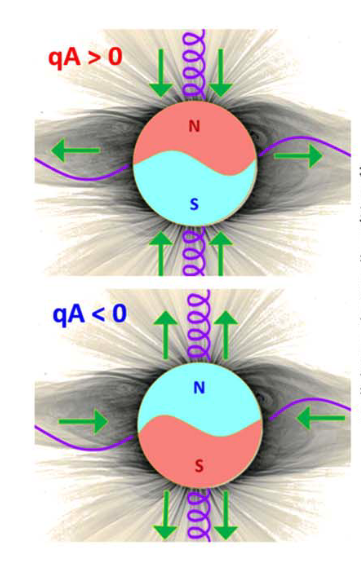
\includegraphics[width = 0.4\textwidth]{images/drift_effect.png}
	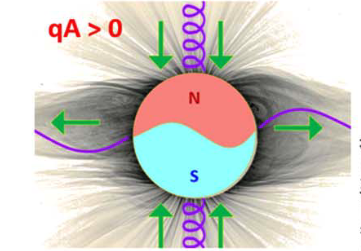
\includegraphics[width = 0.4\textwidth]{images/drift_effect_2.png}
	\caption{The illustration of the drift effects, adapted from the Fig. 4 of \citep{Rankin2022ApJ}}
	\label{Fig:drift_effect}	
\end{figure}

Furthermore, the drift effects which depend on the charge sign and the magnetic polarity are also reflected in the spatial gradient [Vos and Potgieter 2016] of the cosmic rays, including both \ac{GCR} and \ac{ACR}. In this part, we recap the observation of \ac{GCR} particle with energy above hundres MeV\/nuc and the details of the \ac{ACR} component will be discussed in the next section. 

An evidence of \ac{GCR} latitudinal variation is the obseravtion from Ulysses. {Simpson 1995 and Heber 1996a,b} determined a positive variations with an upper limit of 0.25 \% $^\circ$  in the A > 0 solar cycle. When the polarity change to negative, the latitudianl gradient was found to change the sign and decrease to a very small value with a maximum of -0.1 \%$^\circ$.[de simone 2011, Gieseler and Heber 2016]. It was also found that the solar modulation conditions in the same solar polarity but different solar cycle could affect the latitudinal gradient. [Gieseler 2016, Vos potgieter 2018]. What's more the latitudinal gradienst of electron are first time determined by Heber 2008, which is about 0.2 \% $^\circ$ and agree with the proton gradient.

Recently, by revisiting the Helios GCR proton data, Marquate 2019 found that the radial gradient in the inner heliosphere (0.3 - 1 au) is about 6.6 $\pm$ 4 \% \/au, compared with the previous results of 2.5 $\pm$ 0.5 \% \/au between 2 and 28 au [Webber Lockwood 1981]. Such a discrepancy indicates that the radial gradients in the inner helioshphere have different bahaviour than that in the outer heliosphere.

%The spatial gradient, including the latitude and radial gradients have already been observed by multiple missions for the region from 1 AU to the edge of the heliosphere in the past few solar cycles, for instance the two Voyager probes, the Ulysses spacecraft, Pioneer and also combined the measurements like PAMELA from L1 point, [citaion]

\section{Anomalous Cosmic Ray}

\ac{ACR} are mostly the singly charged energetic particle dominated the energy range between few meV/nuc to $\sim$ 100 MeV/nuc. \acs{ACR} were firstly discovered by the \acs{IMP} 7 and 8, the instrumnent back to 1970s \citet{Garcia1973ICRC, Hoverstadt1973PhRvL, McDonald1974ApJ}. By analyzing the lower spectra of cosmic rays, the scientist found an "unusual" enhancement of the flux of helium ($<$ 50 MeV\/nuc), oxygen and nitrogen ($<$ 20 MeV\/nuc) below 100 MeV\/nuc. As the oxygen spectrum which is pointed out by the arrow in Figure \ref{Fig:Oxygen_spectra_cosmic_ray} shown, the intensity of lower energy oxygen did not decrease as the energy decrease from hundred MeV/nuc to MeV/nuc, as expected from our understanding of the \ac{GCR} spectrum, but increase instead. Those particles have been known as the \ac{ACR}. \ac{ACR} elements include helium, nitrogen, oxygen, and neon that have been discovered in the inner heliosphere, and Ar and possibly protons that have been found in the outer region of heliosphere \citet{Klecker1995SSRv}.

It is believe that ACRs are the high energy interstellar pick up ions which are accelerated in termination shock of the heliosphere \citet{Fisk1974ApJ}. The pick up ions are oriented from the intersteallar neutral atoms which are ionzied by the solar UV and the interaction with solar wind ions when they drift into the heliosphere. After being ionized, the solar wind carry those pick up ions and transport them to the outer heliosphere, where the charge particles are accelerated by the blunt termination shocks \citet{McComas2006GeoRL} and gain energy up to few tens of MeV/nuc. Currently , this is the most accepted theory of the ACR origin, which is also supported by the current observation of various instrument \citet{McComas2019ApJ, Cummings2019ICRC}.

One of the key chararcters of \ac{ACR} is that particles are singly charged \citep{Klecker1980GeoRL,Adams1991ApJ, Klecker1995ApJ}. Such property indicates the distinct source as \ac{GCR} and \acp{SEP} and limited travel age of \acp{ACR} in the space. The direct measurement of the charge states of ten of MeV\/nuc particles is quite difficult with the current measurement technique. Therefore, at early stage most works to determine the charge state were based on the propagtion model. For instance, \citet{Klecker1980GeoRL} report that the \ac{ACR} oxygens have lower charge states $<$3 by observing the phase leg effects. Later, a smart method using the Earth's magnetic field as a magnetic spectrometer is applied to determine the charge states. \citet{Adams1991ApJ} and \citet{Klecker1995ApJ} both confirmed the inonic charge of oxygen, nitrogen and neons with the energy around tens MeV/nuc equals to 1.

As we introduced and explained before in the last section, the transport process of the cosmic ray in the heliosphere can be modeled by the TPE equation. The complex processes include diffusion caused by the \ac{HMF} fluctuation, adiabatic energy loss, convection in the expanding solar wind and the drift effects in the large-scale \ac{HMF} which have already been well modeled \citep{Parker1965Pss, Jokipii1977ApJ, Jokipii1981ApJ}.

By 1 AU, similar to \ac{GCR}, the intensities of \ac{ACR} are also heaviely modulated during their transportation in the solar wind and globar \ac{HMF}. Figure \ref{Fig:ACR_solarmodulation} show the comparison between the ACR oxygen intensity and the neutron monitor count rate which is a proxy of the GCR variation in the deep space. The \ac{ACR} intensities show clearly the peaked and plateau-shaped profiles which depend on the magnetic polarity in the last two and half solar cycles, i.e. during the A $<$ 0 period, particle drift into the heliosphere in the equatorial region along the \ac{HCS} and drift outward from the south and north pole region and vice veras during the positive polarity solar cycle.

%Such a trend is consistent with \ac{GCR} and neutron monitor 
%measurement.


\begin{figure}
	\centering
	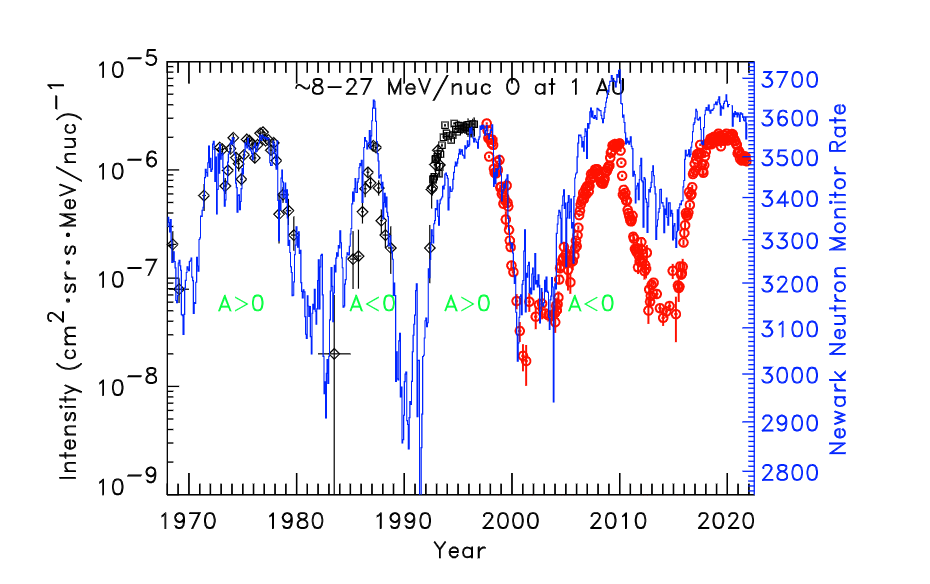
\includegraphics[width = 0.9\textwidth]{images/ACR_solarmodulation.png}
	\caption[Long term variation of \ac{ACR} oxygen and neutron monitor count rate]{ACR oxygen intensity variation with energy between 8 and 27 MeV/nuc at 1 AU measured by ACE/SIS instrument (red) and count rate of Newark Neutron monitor (blue). The blue data points are from the earlier measurements \citep{Mewaldt1993GeoRL}. The plot is adapted from Figure 6 of \citet{Giacalone2022SSRv}}.
	\label{Fig:ACR_solarmodulation}
\end{figure}


As we explained before, the spatial distribution of the \ac{ACR} along the radial and latitudinal direction contains important information of how the particles transport and being accelerated in the heliosphere and out of the helioshphere, i.e. terminaton shock \cite{Rankin2021ApJ}.  Therefore, by determining the magnetitude of the gradient, we can estimate and reconstruct the transport process including drift and diffusion of the \ac{ACR} in the heliosphere. The following general equation is used to model the radial and latitudinal gradients:

\begin{equation}
	\mathrm{ln}(\frac{f_{M}}{f_{E}) = G_r \Delta R  + G_{\theta} \Delta \theta + C
\end{equation}
where $f_{M}$ is the corresponding measurements from the spacecraft away the 1 AU and the equatorial plane; $f_{E}$ is the measurement by missions at 1 AU, for instance SOHO, ACE and so on; $G_r$ and $G_{\theta}$ are the radial and latitudinal gradients respectively. $C$ is the constant.

According to the prediction of the particle transport model and the understanding of the drift effect , the latitudianl gradient changed the sign during different polarity \ac{SC}. The observation evidence of latitudinal gradient of in the outer heliosphere were firstly determined by the two Pioneer and Voyager missions. {Mckibben 1979, Cumming 1987, Chritson 1986}. They found that the lartitudinal gradients of 15 Mev\/nuc \ac{ACR} helium during solar cycle of A > 0, range from 2.1 to 3.1\% $^\circ$ and during A<0 solar cycle, from -2.2 - -1.6 \% \/$^\circ$. While the ACR oxygen have even larger gradient range from -3.7 to -2.9\%\/$^\circ$ {Cumming 1987}.

Later Ulysses mission, operating in the inner heliosphere ($<$ 5 au),  provide the polar region measurement of the cosmic rays, hence including more latitude region (up to 80$^\circ$). Lanzerotti 1995 and Heber 1999 found that in an A >0 solar magnetic period, the latitudinal gradient change between  0.39\% \/$^\circ$ and 2.12 \% \/$^\circ$. However, during the opposite solar polarity, such gradient reduced about 5 times to about -0.3 - 0.4 \% \/$^\circ$, which is consistent with zero. \citep{Cummings2009GeoRL} concluded that particles could not drift into the inner heliosphere along the \ac{HCS} in this solar cycle. Besides, a north-south asymmetry was reported by \citep{Simpson1996}.

While the studies of the radial gradients are still ongoing and discrepancies have been found between the recent measurements in the inner heliosphere \citep{Rankin2021ApJ, Marquardt2018} and the previous studies {webber1981,  Marsden1999} especially the in the inner heliosphere. {Rankin2021ApJ, Rankin2022ApJ, Marquardt2018}, based on the different measurement from Helios and \ac{PSP}, have reported consistent ACR oxygen radial gradient about 45\% \/au during A > 0 solar cycle, which is about 3 times higher than the measurement from Webber1981. More recently Rankin2022ApJ reported the radial gradient of ACR heliul with energy between 4 - 45 MeV/nuc during the last solar minimum (2018-2020), which is about 25$\pm$ 5\% \/au. Similarly, those values are larger than the prior observations by Pineer, Voyager and Ulysses mission \citep{McDonald 2001, Webber1981,  Bastian1981, Mckibben1989, McDonald1987, Cummings1987, Cummings1990}. Such discrepancy is still worth to be further investigated, especially with the new measurement from \ac{SOLO} and \ac{PSP}.




\section{Radiation hazard of energetic particle}


The high energetic particles are one of the deadly hazard for the human body and electronic hardware in the deep space or in the planetary surface like Mars and Moon which are absence of effective protection from the atmoshphere and inner magnetic field.
Those particles damage the \ac{DNA} in our cells when penetrating tissue or organs and have tendency to kill cells therein. Consequencely, high doses of radiation cause Acute Radiation Syndrome (ARS) or Cutaneous Radiation Injuries (CRI), a rapid whole-body responce\footnote{\url{https://www.nrc.gov/about-nrc/radiation/health-effects/high-rad-doses.html}}. Moreover, longer exposure to the radiation environment increase the risk of cancer, even after the mission is over.
On the other hand, the high energy particle could cause the degradation of instruments and permanently or temporally damage the electronic system of the satellite in the space. The failure of instruments is due to the so-called single event events (SEE) which is the change of state of a memory cell or transistor in the electronic devices and caused by the ionizing particles especially the heavy ions.


% https://www.epa.gov/radiation/radiation-health-effects

The radiation hazard of the energetic particles, according to their source, can be seperated into two types: intensive and short term radiation caused by the \ac{SEP} and the long existed but lower intensity radiation caused by the \ac{GCR}.
The large exposures of the intensive radiation could immediately cause the acute radiation syndrome, such as nausea and vomiting. While the chronic exposure to the GCR radiation environment, though not fatal immediately, can increase the probability of late-term consequence, like cancer, damage to the central nervous system and many other side effect \citep{Guo2021AARv, Cucunotta and Durant 2006, Kennedy 2014, Iancu 2018}. 
The variations of radiation dose rate on the Mars surface over the last ten years, are given in Fig.~\ref{Fig:Rad_GCR_radiation}. Apart from the several \acp{SEP} caused abrupt enhancement of the dose rate up to few times higher, the overall dose calculated by the MSL/RAD is increasing from the solar maximum to the solar minimum during the solar cycle 24, due to the solar modulation of the GCR intensity.

Based on the particle energies, we could further divide the soft and hard particles.
As indicating in Fig.~\ref{Fig:SEP-radiation_hazard}, protons of 150 MeV are considered as hard radiation, which energetic enough penetrating 20g/cm2 of aluminium. While the soft protons start from energy of 50 MeV, where proton begin to penetrate spacesuits and the skin of spacecraft \citep{Reames2021LNP}. 


Apart from the above two, the secondary particles like protons, and neutrals generated from the interaction between energetic paritcle and planetary regolith are another signicant contribution of the radiation dose. The secondary protons have enough energy to penetrate the space suite and cause the radiation hazard \citep{Xu2022Frontier}. While the secondary neutrals are even more harmful than the charged particles.
On the lunar surface, according to the simulation, who estimated the radiation hazard of the secondary particles on the lunar surface and found it account for ?\% of the total radiation hazard \citep{Hassler2014}. 

In the future, the potential human mission requires longer stay of astronauts on the planetary surface or in the space when traveling to the destination, which mean the more probability of the exposure to the radiations, no matter insensive one or the background one. Therefore, properly estimation of the radiation hazard in different situation is essential and vital preparation for future human mission.



%Apollo mission not affected by the SEP, 


%Earth is protected by atmosphere and magnetosphere
%Mar not, Lunar not.






\begin{figure}
	\centering
	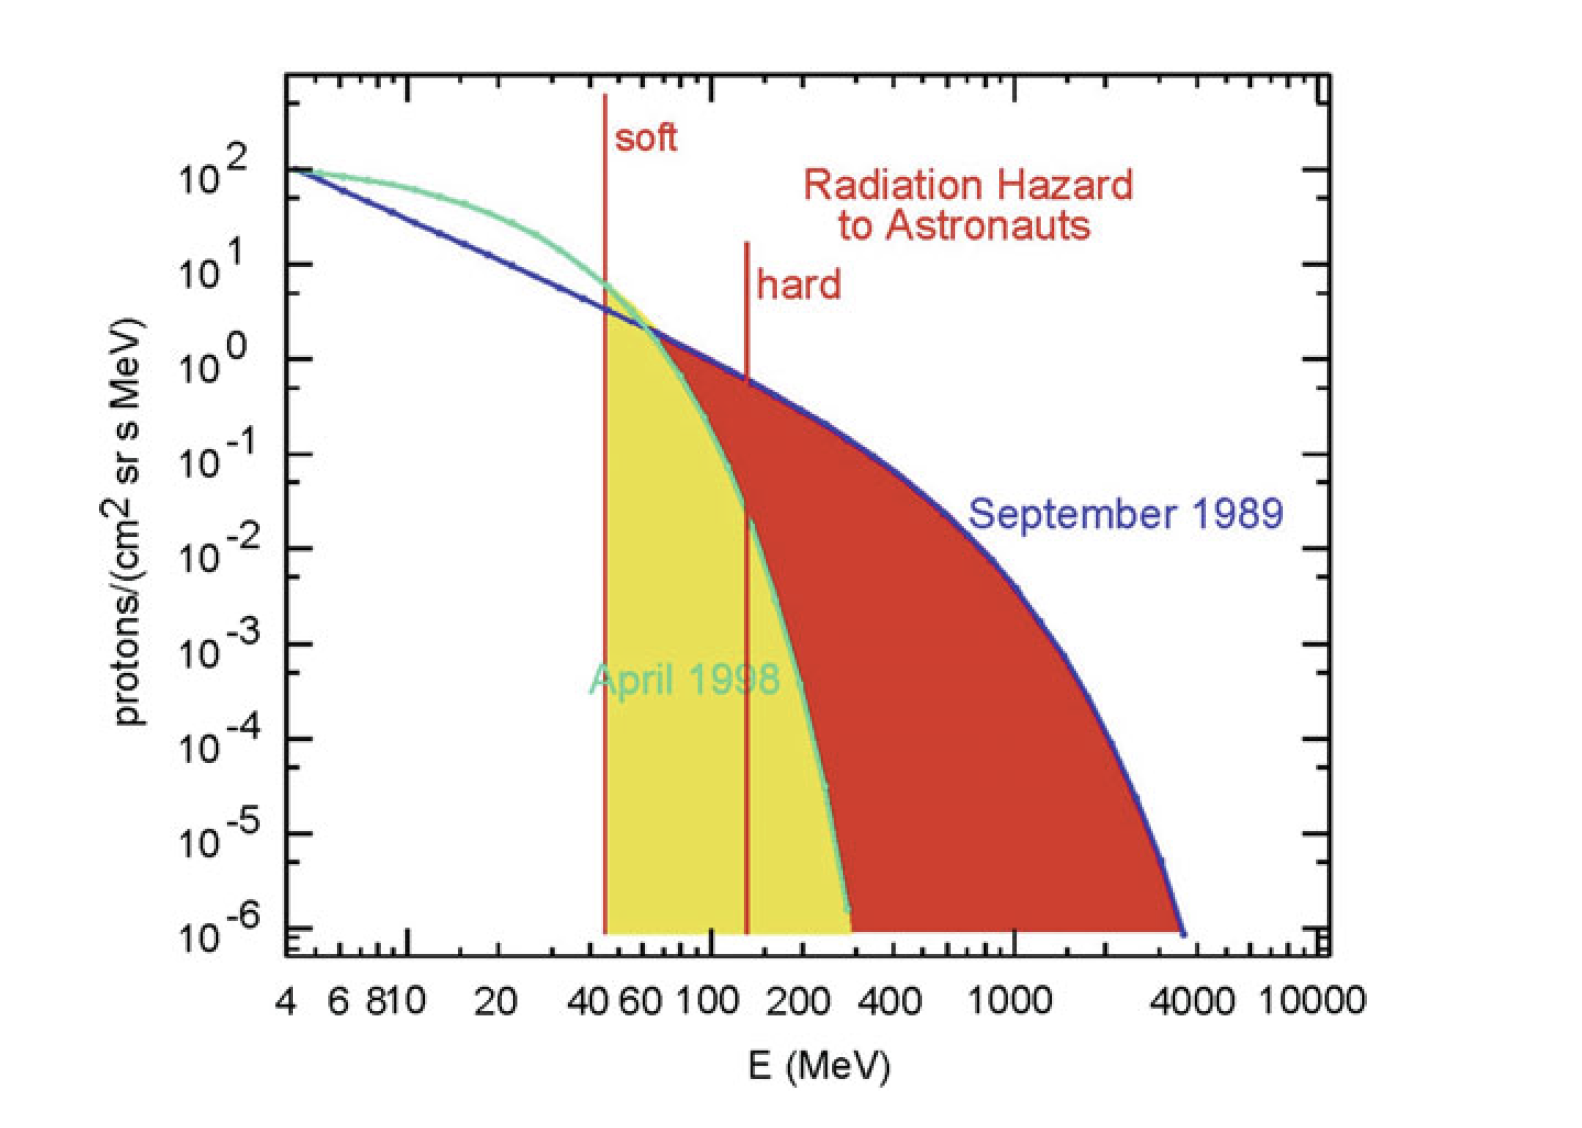
\includegraphics[width = 0.75\textwidth]{images/SEP-radiation_hazard.png}
	\caption[The proton spectra in two SEP events indicating the possible radiation energy]{The proton spectra of two famous SEP events. The shadow regions indicates the energy region of the harmful protons to the instrument and human body. Both "hard" and "soft" spectra threat the human activities. Figure is adapted from \citep{Reames2021LNP}}
	\label{Fig:SEP-radiation_hazard}
\end{figure}
Radiation hazard of the SEP 


\begin{figure}
	\centering
	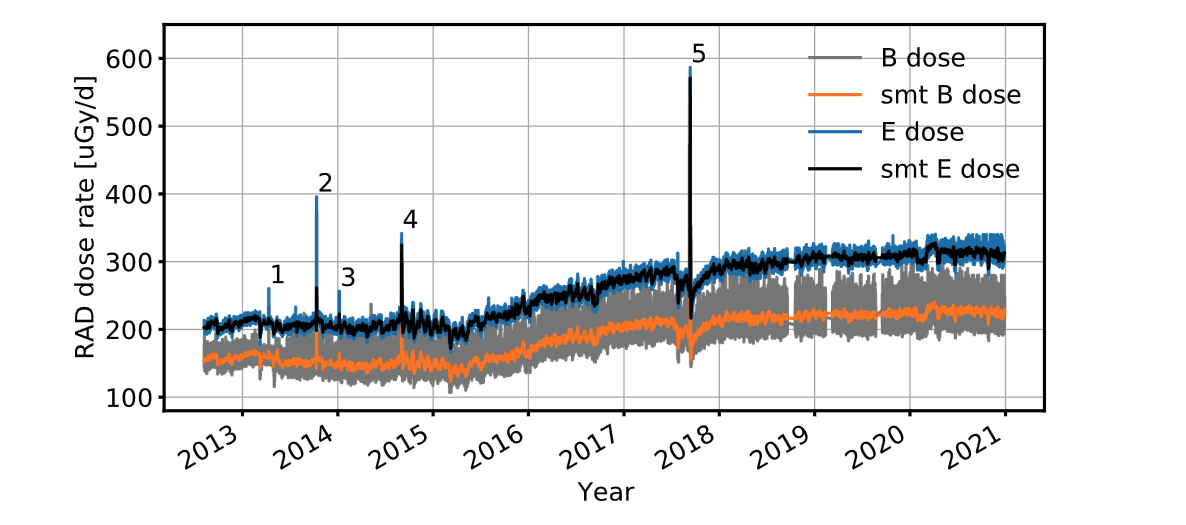
\includegraphics[width = 0.9\textwidth]{images/Rad_GCR_radiation.png}
	\caption{The radiation dose rates on the Martian surface, measured by the \ac{RAD} in the silicon detector B (grey) and plastic detector E (blue). The daily averaged dose rates of B (smt B dose, orange) and E (smt E dose, grey) overlay the original measurements. Apart from 5 prominent SEPs (number 1-5), the long-term trend of dose rate is correlated with the \ac{GCR} variation. The figure is adapted from \citep{Guo2021AARv_rad}}
	\label{Fig:Rad_GCR_radiation}
\end{figure}



\section{Motivition}

The few tens of MeV energy range is an very important energy range for the heliosphere. In this part the SEP, ACR, lower GCR are bothe there. Therefore, more attention required here

New solar Cycle
As ** indicating the solar minimum of SC 23/24 was quite unusual, with a much weaker \ac{HMF} compared with the history record and a higher then ever GCRn intensity. Further more, The recent solar minimum 
is even more unusual, the highest GCR intensity in the history and the unusual ACR intensity [that paper]. 



New measurements, new time and multipoints (NNM)
new age (deep space age)

New instrument, new data, PSP launched, SOLO, LND, and many other missions of different goverment
Such new observation provide valuable data to study the energetic particles
Secondly, as we described above, the solar minimum of SC 23/24 is unusual, and the recent solar minimum is even more unusual, the highest GCR intensity in the history and the unusual ACR intensity [that paper]. Such unusual solar minimum provide a good chance to study the solar modulation of the energetic particles. Special Solar minimum
Furthermore, the radiation hazard of high energy particle is of great interests to the human space exploration. 


Therefore in the following section of the thesis, following the idea of using the totally new measurements from SOLO and LND, we will show the new observation of SEP from the LND, GCR and secondary proton measurement on the Luanr surface, quite time spectra (GCR) measure in the inner heliosphere and the radial gradient change of the ACR helium in the new solar cycles.

% The exploration of space has witnessed a surge in intensity, with an increasing number of countries aspiring to venture into this domain. Noteworthy examples include NASA's initiation of the Artemis mission, which aims to return to the Moon by 2024. Similarly, China has unveiled its plans to establish a lunar base on the lunar surface by the 2030s, while the European Space Agency (ESA) has also embarked on a lunar lander mission. Most recently, a Japanese lunar lander mission was launched; however, it regrettably encountered failure.

% Under these circumstances, the study of solar energetic particles (SEPs) assumes greater significance. SEPs pose a significant radiation hazard for future human exploration on the lunar surface. The most hazardous SEP events have the potential to induce radiation increases of substantial magnitude.

% SEP events directed towards Earth can become an issue of space weather and
% very energetic events can cause a so-called Ground Level Enhancement (GLE).
% This means that the radiation level on the ground increases which can be seen in
% neutron monitor measurements.